% ------------------------------------------------------------------------------
\subsection{PAQ 2 : Le retour}

% ▿▿▿▿▿▿▿▿▿▿▿▿▿▿▿▿▿▿▿▿▿▿▿▿▿▿▿▿▿▿▿▿▿▿▿▿▿▿▿▿▿▿▿▿▿▿▿▿▿▿▿▿▿▿▿▿▿▿▿▿▿▿▿▿▿▿▿▿▿▿▿▿▿▿▿▿▿▿
\begin{frame}
\tableofcontents[subsectionstyle=show/shaded/hide, subsubsectionstyle=hide, sectionstyle=show/hide]
\end{frame}
% ▵▵▵▵▵▵▵▵▵▵▵▵▵▵▵▵▵▵▵▵▵▵▵▵▵▵▵▵▵▵▵▵▵▵▵▵▵▵▵▵▵▵▵▵▵▵▵▵▵▵▵▵▵▵▵▵▵▵▵▵▵▵▵▵▵▵▵▵▵▵▵▵▵▵▵▵▵▵

% ▿▿▿▿▿▿▿▿▿▿▿▿▿▿▿▿▿▿▿▿▿▿▿▿▿▿▿▿▿▿▿▿▿▿▿▿▿▿▿▿▿▿▿▿▿▿▿▿▿▿▿▿▿▿▿▿▿▿▿▿▿▿▿▿▿▿▿▿▿▿▿▿▿▿▿▿▿▿
\begin{frame}[allowframebreaks]
\frametitle{Pourquoi un nouveau PAQ ?}

\begin{block}{Rebondir} % Sur le précédent paq
\begin{itemize}
	\item Leçons tirées du PAQ précédent % Manque de précisions : réunions, moyens de communication
	\item Petits problèmes à 4 => gros problèmes à 8 % Organisation
\end{itemize}
\end{block} % Fin du block [Rebondir]

\begin{block}{Documenter}
\begin{itemize}
    \item \emph{Mise en bouche} avant de rentrer dans le projet % Abréviations
    \item Méthodologie % Comprendre la méthodologgie => comprendre la conception du projet
    \item Garanties pour le client, support de communication, ...
    \item Requis par le cahier des charges
\end{itemize}
\end{block}

\begin{block}{Une référence}
\begin{itemize}
    \item Pour le groupe % Pour savoir comment s'organiser, quels outils utiliser
    \item Reprise du projet % Abbréviations et outils notemment
\end{itemize}
\end{block}

\end{frame} % Fin de la frame [Pourquoi un nouveau PAQ ?]
% ▵▵▵▵▵▵▵▵▵▵▵▵▵▵▵▵▵▵▵▵▵▵▵▵▵▵▵▵▵▵▵▵▵▵▵▵▵▵▵▵▵▵▵▵▵▵▵▵▵▵▵▵▵▵▵▵▵▵▵▵▵▵▵▵▵▵▵▵▵▵▵▵▵▵▵▵▵▵

% ▿▿▿▿▿▿▿▿▿▿▿▿▿▿▿▿▿▿▿▿▿▿▿▿▿▿▿▿▿▿▿▿▿▿▿▿▿▿▿▿▿▿▿▿▿▿▿▿▿▿▿▿▿▿▿▿▿▿▿▿▿▿▿▿▿▿▿▿▿▿▿▿▿▿▿▿▿▿
\begin{frame}
\frametitle{Principales différences avec le premier}

\begin{block}{Ajouts}
\begin{itemize}
	\item Communication % Mailing list pour que tout le monde soit informé des changements + ICE tel
	\item Chainage des tâches % Quand on a fini, on prévient
	\item Chaine de responsabilité % Pour savoir comment faire remonter les problèmes
\end{itemize}
\end{block} % Fin du block [Ajouts]

\begin{block}{Modifications}
\begin{itemize}
	\item Binômes % Fusion des groupes
	\item Réunions % 3/semaine => bilan + organisation
	\item Arborescence % Maintenant plus précise
	\item Nomenclature % Parce que c'était pas assez précis
	\item Outils % Pas le même 'projet' => besoins différents; plus nombreux => on oublie Libreoffice qui n'est pas versionnable (binaire car compressé)
\end{itemize}
\end{block} % Fin du block [Modifications]

\end{frame} % Fin de la frame [Principales différences avec le premier]
% ▵▵▵▵▵▵▵▵▵▵▵▵▵▵▵▵▵▵▵▵▵▵▵▵▵▵▵▵▵▵▵▵▵▵▵▵▵▵▵▵▵▵▵▵▵▵▵▵▵▵▵▵▵▵▵▵▵▵▵▵▵▵▵▵▵▵▵▵▵▵▵▵▵▵▵▵▵▵

% ▿▿▿▿▿▿▿▿▿▿▿▿▿▿▿▿▿▿▿▿▿▿▿▿▿▿▿▿▿▿▿▿▿▿▿▿▿▿▿▿▿▿▿▿▿▿▿▿▿▿▿▿▿▿▿▿▿▿▿▿▿▿▿▿▿▿▿▿▿▿▿▿▿▿▿▿▿▿
\begin{frame}
\frametitle{Outils utilisés}

\begin{block}{Les retirés}
\begin{itemize}
    \item LibreOffice % Difficultés avec le git, rendus pas exceptionnels
\end{itemize}
\end{block}

\begin{block}{Les nouveaux}
\begin{itemize}
    \item \LaTeX % Modularite + fichier textes (dépôt git)
    \item Dia % Pour certains diagrammes
    \item Inkscape % Pour la norme graphique
    \item Qt % Pour développement
    \item SQLite \& MySQL % SQLite pour premizes tests, MySQL parce que demandé par cdcf
    \item Windows % Pour tests de compatibilité
\end{itemize}
\end{block}

\end{frame} % Fin de la frame [Outils utilisés]
% ▵▵▵▵▵▵▵▵▵▵▵▵▵▵▵▵▵▵▵▵▵▵▵▵▵▵▵▵▵▵▵▵▵▵▵▵▵▵▵▵▵▵▵▵▵▵▵▵▵▵▵▵▵▵▵▵▵▵▵▵▵▵▵▵▵▵▵▵▵▵▵▵▵▵▵▵▵▵

% ▿▿▿▿▿▿▿▿▿▿▿▿▿▿▿▿▿▿▿▿▿▿▿▿▿▿▿▿▿▿▿▿▿▿▿▿▿▿▿▿▿▿▿▿▿▿▿▿▿▿▿▿▿▿▿▿▿▿▿▿▿▿▿▿▿▿▿▿▿▿▿▿▿▿▿▿▿▿
\begin{frame}
\frametitle{Charte graphique : Avant}

% Parce que on en avait pu quand on est passé à latex

\begin{figure}
   \begin{minipage}[c]{.4\linewidth}
      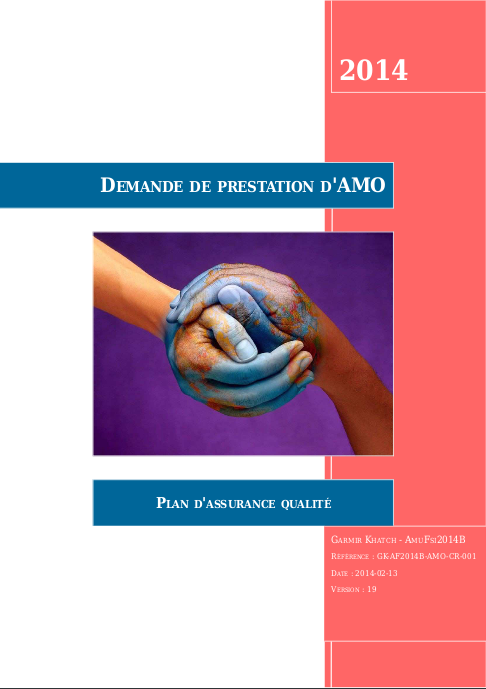
\includegraphics[width=\textwidth]{Images/cg_entete_avant.png}
   \end{minipage} \hfill
   \begin{minipage}[c]{.4\linewidth}
      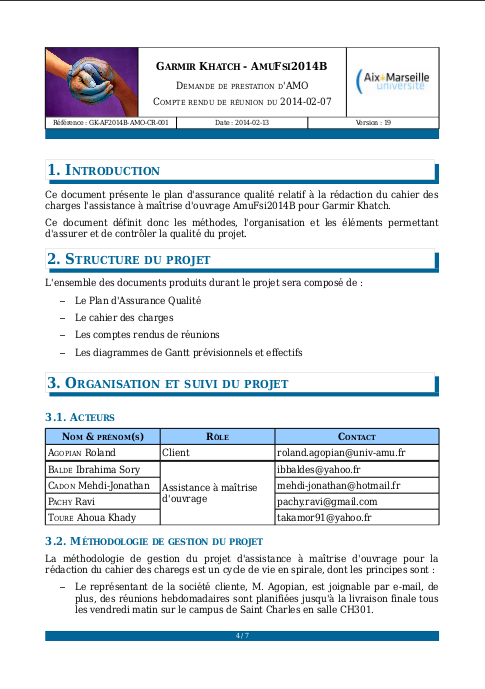
\includegraphics[width=\textwidth]{Images/cg_corps_avant.png}
   \end{minipage}
\end{figure}

\end{frame} % Fin de la frame [Charte graphique]
% ▵▵▵▵▵▵▵▵▵▵▵▵▵▵▵▵▵▵▵▵▵▵▵▵▵▵▵▵▵▵▵▵▵▵▵▵▵▵▵▵▵▵▵▵▵▵▵▵▵▵▵▵▵▵▵▵▵▵▵▵▵▵▵▵▵▵▵▵▵▵▵▵▵▵▵▵▵▵

% ▿▿▿▿▿▿▿▿▿▿▿▿▿▿▿▿▿▿▿▿▿▿▿▿▿▿▿▿▿▿▿▿▿▿▿▿▿▿▿▿▿▿▿▿▿▿▿▿▿▿▿▿▿▿▿▿▿▿▿▿▿▿▿▿▿▿▿▿▿▿▿▿▿▿▿▿▿▿
\begin{frame}
\frametitle{Bilan du (nouveau) PAQ}

\begin{block}{+}
\begin{itemize}
	\item Bases du premier PAQ % Les leçons ont été bénéfiques
	\item Plus utilisé % Pour se mettre d'accord sur outils, arborescence, nomenclature
	\item Plus complet % Après les ajouts et modifications apportés
\end{itemize}
\end{block} % Fin du block [+]

\begin{block}{-}
\begin{itemize}
	\item Complétion constante % Parce qu'on était loin de penser à tout dès le début
	\item Pas toujours facile à suivre % Binomes
\end{itemize}
\end{block} % Fin du block [-]

\end{frame} % Fin de la frame [Bilan du (nouveau) PAQ]
% ▵▵▵▵▵▵▵▵▵▵▵▵▵▵▵▵▵▵▵▵▵▵▵▵▵▵▵▵▵▵▵▵▵▵▵▵▵▵▵▵▵▵▵▵▵▵▵▵▵▵▵▵▵▵▵▵▵▵▵▵▵▵▵▵▵▵▵▵▵▵▵▵▵▵▵▵▵▵

% Fin de la sous-section [PLan d'Assurance Qualité]
% ------------------------------------------------------------------------------

